% !TEX root = ../notes_template.tex
\chapter{Fick's Equation}\label{chp:fick_equation}
Updated on \today
\minitoc

% Hi Nathaniel - anything with a % in front of it is a comment and doesn't get compiled as text into the book. Use it as necessary to leave questions for me or reminders for yourself. Also - at the moment this chapter is not added to the compile list. It won't show up in the PDF until I add it to the file called "book.tex". If you want to see how its compiling you could remove the "%" in front of the reference to it in the "book.tex" file and hit recompile.

This chapter introduces Fick's equation as a model to connect the muscle and supporting systems roles in attaining and sustaining activity.

% Just the equation for the sake of having it to copy/paste where ever it is needed in the chapter
\begin{equation}
    \dot{V}O_2 = \dot{Q} \cdot (a-v)O_2
\end{equation}



\vspace{5mm}

\textbf{Objectives include:}
\begin{enumerate}
    \item Define Fick's equation and recognize the relevance 
    \item Review the determinants of cardiac output and how the comprising variables may 
    \item
    \item
    \item
    \item
\end{enumerate}


Fick's equation offers a method to determine substance consumption using a set of known variables: 

\begin{enumerate}
    \item Flow rate to an organ/system
    \item The concentration of substance in the arterial blood entering the organ
    \item The concentration  of substance in the venous blood leaving the organ
\end{enumerate}

Specific to Fick’s equation, the substance in question is most typically oxygen. Thus, the necessary components to calculate and apply Fick’s equation relevant to this area of study are as followed:

\begin{enumerate}
    \item Flow rate to an organ/system (cardiac output)
    \item The concentration of oxygen in the arterial blood entering the organ (arterial oxygen concentration, CaO2)
    \item The concentration  of oxygen in the venous blood leaving the organ (venous oxygen concentration, CvO2)
\end{enumerate}

Using these variables, Fick’s equation can be formatted as:

\begin{equation}
    \dot{V}O_2 = \dot{Q} \cdot (a-v)O_2
\end{equation}

Where: 

\begin{itemize}
    \item VO2 = the amount of oxygen taken up by the system or organ
\end{itemize}
\begin{itemize}
    \item Q = cardiac output
\end{itemize}
\begin{itemize}
    \item avO2 difference = the difference in oxygen concentration between the arterial and venous blood (CaO2 - CvO2)
\end{itemize}

In contrast to determining the VO2 using Fick’s equation, another variation of this equation can be used to determine the cardiac output. A simple rearrangement of the equation would yield:

Q = VO2/ avO2 difference 

\begin{equation}
    \dot{Q} = \dot{V}O_2 / (a-v)O_2
\end{equation}

Fick’s equation can be applied systemically (e.g. determining oxygen consumption of the whole system) or at a more local area of the body. For example, Fick’s equation can be used to calculate oxygen consumption specifically to the myocardium using the following variables: 

MVO2 = CBF x (CaO2 x CvO2) 

\begin{equation}
    \dot{MV}O_2 = \dot{CBF} \cdot (CaO_2)(CvO_2)
\end{equation}

Where:
MVO2 = myocardial oxygen consumption
CBF = coronary blood flow
CaO2 = arterial oxygen content
CVO2 = venous oxygen content

It may seem that in the role of the physical therapist, it is not clinically necessary to establish these values as it does not directly pertain to our intervention and/or examination selection. 

Nevertheless, Fick’s equation offers benefit as it lends an understanding as to how flow rate, oxygen consumption, and the difference in arterial and venous oxygen concentration may change under situations which alter homeostatic conditions. The role of this chapter is to look at the determinants of each of the variables in Fick's equation and to understand the interplay of systems that can influence the variables. 

Oxygen consumption is a highly integrated physiological variable and is ultimately determined by the three variables in the Fick equation: cardiac output, arterial oxygen content, and venous oxygen content. As will be seen later in the chapter, these variables are influenced by a number of factors and are constantly monitored and then subsequently adjusted to maintain the equilibrium of each individual system and the body at large. 


\section{Determinants of Cardiac Output}
To begin, this section of the chapter outlines the determinants of cardiac output and evaluates how they can change under varying physiological circumstances. As described in Chapter 7, cardiac output is defined as the volume of blood pumped out by each ventricle per unit of time (one minute). 

The equation for cardiac output is Q = SV x HR. Stroke volume is the product of the left ventricle ejection fraction (LVEF) and the end diastolic volume (EDV), also known as preload. Therefore, Q = SV x HR can be further broken down into: 
 \begin{equation}
    \dot{Q} = (LVEF \cdot EDV) \cdot HR
\end{equation}

 As such, the main determinants of cardiac output are as follows:
1. Heart Rate
2. Stroke Volume (EDV and LVEF) 

Based on the equation (and under stable conditions, i.e. the other variables do not decrease proportionally), increases in any of the above-mentioned variables (LVEF, EDV, or HR) will result in an increased cardiac output and thus, increased systemic and/or localized blood flow. Similarly, decreases in the aforementioned variables without compensatory changes will lower cardiac output. These concepts will be explored later in the text. 

In order for the heart to impart blood effectively through the systemic vasculature, it is imperative that the above physiological characteristics work synergistically. When this synergy is compromised homeostasis is endangered, and pathology can arise. But it is important to remember that these compensatory systems do not only exist in the presence of pathology, but rather, are constantly monitoring and subsequently adjusting variables to accommodate for the changes in homeostasis. 

\textbf{Integrative Exercise: Brachial Blood Pressure During the Supine to Sit Transfer:}
A common, non-pathological integration of the cardiac output determinants  (Q, HR, SV) is seen every time a non-pathological patient performs a functional transfer, like the transition from supine to sitting. In a supine position blood flow is evenly distributed throughout the body secondary to the lack of gravity related pressure changes. With the transition to a sitting position, the effect of gravity redistributes blood from the upper torso and extremities into the lower body, which can create a transient decrease in stroke volume due an attenuated venous return. To combat the initial decrease in cardiac output the body (via the baroreceptor reflex) will increase heart rate and venous return mechanisms, therefore normalizing the cardiac output. 

We will begin by evaluating how heart rate may influence cardiac output beyond acting as a direct multiplier in the equation. 

\subsection{Heart Rate}
How might changes in heart rate affect cardiac output? Aside from being a direct multiplier in the equation, heart rate can also have a direct effect on stroke volume (the other multiplier in the cardiac output equation). More specifically, changes in heart rate, whether increased (tachycardia) or decreased (bradycardia) can influence the stroke volume through modulation of diastolic filling time and therefore end diastolic volume. In an otherwise uncompensated state, bradycardia will increase cardiac contractility while tachycardia will decrease cardiac contractility - both achieved via the Frank Starling Mechanism.  More specifically, under bradycardic conditions there is a greater amount of time in-between each myocardial contraction for blood to fill into the left ventricle, which increases end diastolic volume and subsequently, stroke volume. Although this is true in isolated conditions, the effect of heart rate on stroke volume must be examined relative to the cardiac conditions currently present. In other words, under homeostatic conditions these variables rarely change without integrated, multi-variable compensations, which can exist under both acute and chronic circumstances.  Factors such as nervous system activity, hormonal influences, underlying medical/health conditions, and metabolic needs all can influence heart rate and subsequently cardiac output. This concept can be explored more broadly in the context of Fick's equation when evaluating the compensatory mechanisms at play when having a patient undergo a bout of aerobic exercise. 

\paragraph{Integrative Exercise: Heart Rate and Progressive Aerobic Exercise: How are the variables in Fick's Equation affected in a patient that is acutely progressing through a bout of aerobic exercise? What are the drivers for an increase in oxygen consumption with this task?}
An example of the interplay between the multipliers in the cardiac output equation can be seen during a graded exercise program. As a patient gradually increases their exercise workload it is expected to see an elevation in heart rate to meet the metabolic demands of the exercising skeletal muscle. In an otherwise uncompensated state this elevation in heart rate would decrease stroke volume secondary to a decreased diastolic filling time. But, due to the complex multi-system response, it is much more likely to see an increase in stroke volume (see Figure 1.). This increase in stroke volume paired with the elevated heart rate creates a net increase in cardiac output that is typical of a patient acutely increasing there physical activity. This simple example highlights that changes to one variable do not occur in isolation. The body is constantly adapting and adjusting variables across all systems to meet the internal requirements (e.g. elevated metabolic needs) from the external demands (e.g. aerobic exercise). 

\begin{figure}
    \centering
    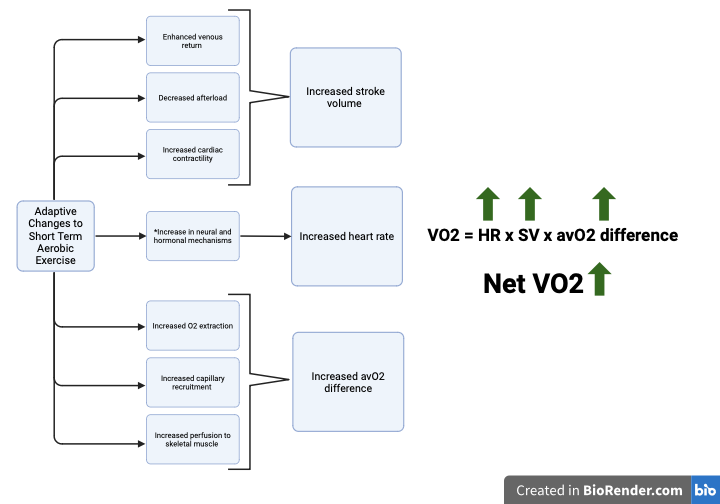
\includegraphics[width=0.5\linewidth]{Short Term Adaptive Changes.png}
    \caption{Figure 1. Short Term Adaptation to Aerobic Exercise}
   \label{fig:enter-label}
   \caption{*Neurohormonal Mechanisms: 
1. Sympathetic activation 
    -Stimulation of cardiovascular control centers in the brain 
2. Parasympathetic withdrawal 
    -Reduced vagal tone 
3. Catecholamine release 
    -Epi, NE 
}
\end{figure} 
As compared to stroke volume, heart rate operates at a wider range of what is generally considered physiologically safe. That is to say, stroke volume tends to remain within a more narrow, well-controlled range. As heart rate is primarily influenced by neural mechanisms (i.e. the response of the autonomic nervous system), this variable can be readily adjusted to accommodate for alterations in homeostasis. As we will look at later in the chapter, stroke volume is predominantly dependent on mechanical factors (e.g. preload, afterload, and contractility), which is unlikely to occur prior to the aforementioned neural response. Heart rate may very well be considered the body's first line of defense in managing changes in cardiovascular homeostasis. 



\begin{figure}



    \centering
    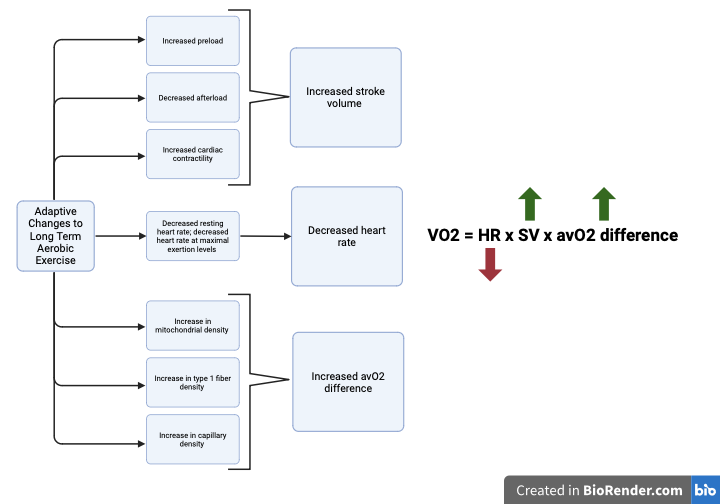
\includegraphics[width=0.5\linewidth]{FicksChronicAerobic.png}
    \caption{Figure 2. Long Term Adaptations to Aerobic Exercise}
    \label{fig:enter-label}
\end{figure}

This acute bout of exercise where all variables in Fick's equation are increased can be compared to the long term adaptive changes seen accompanying a long term aerobic training program. Compared to the integrated cardiac response to acute exercise, long term adaptations result in all variables increasing with the exception of heart rate, which has a net decrease. 

These %Figure 1. --> reasons SV increases when exercising 
Under what situations may bradycardia decrease stroke volume? 
1. Poor ventricular filling time 
2. Poor ventricular contractility 
3. Reduced preload 
4. Increased afterload 
5. Autnomic imbalance 
Under what situations may tachycardia decrease cardiac output?
E.g. Reflex bradycardia with subsequent  hemodynamic instability. 


As we will look at shortly, end diastolic volume is the most important determinant of stroke volume. With this known, heart rate should be recognized as a major determinant in stroke volume and thus cardiac output. Look at the situations below to further explore how fluctuations in heart rate may affect cardiac output. 


and has a significant  as it relates to the body's ability to make an intelligent and efficient offsetting response.

Under what conditions may bradycardia increase stroke volume? 
E.g. Exercise 
1. 



\subsection{Stroke Volume}

Stroke Volume is defined as the volume of blood ejected during one ventricular contraction. 

\begin{equation}
    SV = EDV \cdot LVEF
\end{equation}

The variables of the stroke volume equation (EDV and ESV) are primarily influenced by three variables: 
\begin{itemize}
    \item Preload
    \item Afterload
    \item Contractility
\end{itemize}

Independently, these variables can all increase (or decrease) stroke volume, but often work cooperatively to alter the amount of blood ejected per contraction to ensure physiological needs are attained and sustained. 

First, we will look at these determinants of stroke volume in isolation and then review the interactions between them. 

\subsubsection{\textbf{Preload}} 

Preload is defined as the volume of blood present in the ventricle following the end of the diastolic phase. Fundamentally, the more blood present in the atrium prior to the systolic phase of the cardiac cycle, the higher the stroke volume. They're a number of mechanisms in which preload is shaped including mechanical, neural, hormonal, and  

\paragraph{Increased venous blood volume}
An increased volume of blood present in venous circulation will produce a greater return to the heart resulting in a greater preload, stroke volume, and cardiac output. 

\paragraph{Venoconstriction and rhythmic skeletal muscle contraction}: 
Arteries and veins are innately unique as compared to one another in that veins have valves whereas arteries do not. The purpose of these valves are to prevent back flow. If veins venoconstrict, blood can only move in one direction - forward (moving proximal back to the heart to increase preload and thus, stroke volume). Increasing the internal radius of the veins would only reinforce their role as a reservoir for the blood. 

\paragraph{Atrial kick}: 
Although diastole occurs through primarily passive flow from an area of high pressure (blood filled atria) to low pressure (ventricle), the atrial contraction that occurs at the end of the diastole results in a transient increase in atrial chamber pressure, which creates a greater pressure gradient between the atria and ventricle. This increased pressure gradient results in the further filling of blood left over in the atria that would otherwise be left due to the lack of a large enough pressure gradient.  

\paragraph{Prolonged ventricular diastole}
The prolonging of time in between ventricular diastole allows for an increase in the relaxation phase of the cardiac cycle. This extended relaxation phase allows a greater volume of blood able to enter the ventricle before ventricular contraction. A greater volume of blood prior to the systolic phase means increased preload, increased preload means increased stroke volume.  

\paragraph{Respiratory pump/decreased intrathoracic pressure, increased abdominal pressure (e.g. deep inhalation):} The respiratory pump (diaphragm) can mechanically affect preload by adjusting the influencing the volume inside the thoracic cavity. As the diaphragm contracts it flattens and descends, thereby increasing the volume in the thoracic cavity (decreasing intrathoracic pressure). It is this decrease in intrathoracic pressure that facilitates the expansion and filling of the pulmonary and abdominal veins. 

\textbf{
\subsubsection{Afterload}

Afterload is the pressure that a chamber must overcome to cause blood to flow out of the chamber. Under stable, uncompensated states, afterload has an inversely proportional relationship to stroke volume (i.e. if afterload is increased, stroke volume and thus cardiac output will be decreased). The three primary factors influencing afterload: 
\begin{itemize}
    \item Vessel radius: refer to Poiseuille's Equation 
    \item Arterial compliance (distensibility of arterial vasculature): denoting how the volume of blood within a vessel changes for a given change in pressure.

\begin{equation}
    C = V/P 
\end{equation}
    \begin{itemize}
        \item C = V/P 
        \item Where: 
        \item C = Compliance (mL/mmHg) 
        \item V = Volume (mL) 
        \item P = Pressure 


\textbf{Blood viscosity:} Resistance to blood flow is directly related to the blood viscosity and is related to the friction created by the interaction between the solvent (fluid molecules in the plasma, related solutes (e.g. RBC’s and proteins), and the vessel wall. Increases in blood viscosity will oppose blood flow, which can create changes in hemodynamic stability. In an otherwise unperturbed state, blood viscosity remains a rather stable variable, though can be affected in changes in hematocrit, temperature, and systemic flow. 

\textbf{Arterial Impedance: }
There is an inverse relationship between vessel radius and internal resistance. Atherosclerotic build up results in a reduction in vessel diameter, which increases the pressure required to achieve consistent flow through the vasculature. It is this increase in pressure that reflects an increased afterload. Example: it may be common to find higher arterial pressures in the elderly as the natural aging process creates a reduction of vessel capacitance. At a lower compliance an increased pressure gradient (increased arterial pressure) must be present to maintain consistent flow through the artery. 
    \end{itemize}
    \end{itemize}

\subsubsection{Contractility}

An increase in cardiac contractility will result in an increased stroke volume for a given preload and afterload. This will present as an increased cardiac ejection fraction as a larger proportion of the given end diastolic volume will be ejected from the ventricle due to the increased pressure gradient created by the increased cardiac contractility. 

Factors increasing ventricular contractility 
\begin{itemize}
    \item Inotropic medication (e.g. cardiac glycosides) 
    \begin{itemize}
        \item Inotropic medications, like Digoxin, can be used to improve cardiac contractility through the primary mechanism of increasing intracellular calcium released by the sarcoplasmic reticulum. 
    \end{itemize}
    \item Sympathetic activation (e.g. release of catecholamines): Among the many effects of an increased sympathetic drive, a increase in cardiac contractility is seen by way of neurotransmitter release and heightened calcium availability.
    \item Parasympathetic inhibition: the role of the parasympathetic nervous system is mitigate the potential stressors to the body (rest and digest) and acts as the antagonist to the sympathetic nervous system. Parasympathetic inhibition (which can occur with a certain class of medications, like anticholinergics) reduce the influence of the parasympathetic nervous system, which creates a relative increase in the influence of the sympathetic nervous system. 
    \begin{itemize}
    \end{itemize}
    \item Afterload via the Anrep Effects
    \item Heart rate via the Bowditch Effect
    \item left ventricular end diastolic volume
    \item Presence of calcium 



\textbf{Integrative Exercise: Chronic Dilated Cardiomyopathy }

Cardiomyopathies are categorically defined as diseases of the heart resulting in cardiac dysfunction. Dilated cardiomyopathy (DCM) is characterized by enlargement of the one or both of the ventricular chambers with an associated compromise in cardiac contractility. Clinically, this may manifest as excessive dyspnea at rest or with exertion, palpitations, heart murmur, and fluid accumulation in the lower extremities and/or abdominal region. 


As compared to a healthy functioning heart, a patient with chronic dilated cardiomyopathy will likely display a decrease in cardiac output (Q) secondary to the enlarged ventricular chamber(s). Among other changes, this enlargement creates a misalignment of myocardial sarcomeric proteins, which influences the heart's ability to productively impart the force required to attain and sustain appropriate systemic flow. In other words, the heart is unable to generate enough force per beat to completely empty the chamber following the systolic phase of the cardiac cycle. As such, an increase in the blood present in the left ventricle following systole is often seen (i.e. increased EDV). But, as compared to what was previously discussed with preload in which an increased EDV brings about an increase in cardiac contractility (via the Frank Starling Mechanism), a heart with dilated ventricular chambers is unable to create the required pressure to advance blood into the next constituent of the circulatory system. So, how might the body compensate to meet metabolic demands (i.e. oxygen consumption needs)? To answer this, we can again look to the other variables comprising Fick's equation \begin{equation}
    \dot{V}O_2 = \dot{Q} \cdot (a-v)O_2
\end{equation}
An increase in cardiac contractility will result in an increased stroke volume for a given preload and afterload. On the contrary, a decrease in cardiac contractility will result in a decreased stroke volume for a given preload and afterload. As stated above, one of the principle pathophysiological characteristics of DCM is a decrease in cardiac contractility, thus decreasing stroke volume and cardiac output. With this decrease in Q, there is a net decrease in oxygen delivery to the tissues, 


\section{Determinants of Arterial Oxygen Content}

The primary determinants of arterial O2 are pulmonary ventilation and pulmonary respiration. As a reminder, 

\subsection{Pulmonary Ventilation}
Pulmonary ventilation is predominantly a function of respiratory rate (the number of breaths taken per unit of time - typically one minute) and tidal volume (the volume of air in a normal inspiration and expiration cycle). As such, any situation that influences either respiratory rate and/or tidal volume will affect pulmonary ventilation, arterial oxygen content, and thus that avO2 difference as a part of Fick's equation. The avO2 difference can be altered in conditions that alter the compliance of the lungs, like restrictive lung diseases, in which the compliance of lungs is decreased secondary to the decrease in lung elasticity. 

\subsection{Pulmonary Respiration}
Pulmonary respiration is primarily a function of three variables: alveolar ventilation, O2 and CO2 pressure differentials, and anatomical and physiological dead space. 

As a reminder, in the upright lung there is a non-uniformity between ventilation and perfusion due to the effects of gravity. This non-uniformity is expressed in regional variations in blood flow to different areas of the lung. Perfusion is highest at the base and lowest at the apex while ventilation is lower at the apex and higher at the base. Alterations in either the perfusion and/or ventilation will result in a V/Q mismatch, which may manifest as dead space or shunt. In both situations, whether dead space or shunt, arterial oxygen content is affected by the alterations to the ventilation or perfusion to the alveoli. 

Below are examples highlighting how arterial oxygen content may be affected based on varying physiological conditions involving changes to  pulmonary ventilation and/or pulmonary respiration.  

\textbf{Integrative Exercise: Hyperkyphosis and Poor Chest Wall Compliance}
Ankylosing spondylitis is an inflammatory arthropathic condition resulting in a gradual worsening of spinal mobility and chest wall excursion. This condition often presents clinically in individuals with excessive thoracic kyphosis, forward head posture, and spinal pain. Individuals with ankylosing spondylitis may also experience changes in lung mechanics and impaired respiratory muscle function secondary to spinal/chest wall hypomobility and skeletal muscle deconditioning (e.g. intercostals and diaphragm). The combined changes characteristic of this condition can have serious implications as it relates to these patients oxygen consumption (VO2). More specifically, distortions in the chest wall and thoracic spine mobility result in decreased ventilation relative to pulmonary perfusion (decreased V/Q ratio) and increase PA-aO2 gradient. In other words, there is no change in the patient’s pulmonary perfusion, but due to reduced compliance of the chest wall and hypomobility of the thoracic spine they're limitations in full lung excursion (most notably, inhalation), which drives the reduction in pulmonary ventilation. As a result of the lower concentration of arterial O2, there is less oxygen available to be delivered to the tissues leading to the likely reduction in VO2. This individual would require greater ventilation in order to reach a given amount of O2. This may manifest clinically as a patient increasing their respiratory rate and tidal volume by taking a greater number of breaths per minute and attempting to increase the amount of oxygen taken in per breath.

\textbf{Integrative Exercise: Pneumonia}
How would pneumonia affect V/Q matching and what compensatory mechanisms may be present to address this change? 

A defining characteristic of pneumonia is the inflammatory response in pulmonary tissue as to combat the offending agent or organism. The inflammatory response brings fluid, which occupies areas of the compromised space (e.g. at the level of the lobe or more distal in the bronchioles and alveoli). This fluid accumulation may manifest clinically in patients who demonstrate and/or complain of pleuritic chest pain, dyspnea, and/or a hacking, productive cough. At a physiological level, the fluid accumulation in the lung will likely decrease the lungs capacity for pulmonary ventilation, therefore a decrease in capillary O2 content. Thus, a decrease in V/Q matching is typically seen as ventilation is decreased, but perfusion is unchanged. 


\textbf{Integrative Exercise: Aortic valve stenosis and Left Ventricular Hypertrophy }
What is the mechanism underlying the adaptive changes to the left ventricular in a patient with aortic valve stenosis? How are the components of Fick’s equation changed in a patient with left ventricular hypertrophy? 

Aortic valve stenosis is defined as a narrowing of the valve separating the left ventricle and aorta resulting in a reduction in cardiac output. In an effort to normalize the cardiac output, increased pressure from the left ventricle must be generated, thus increasing the pressure gradient between these two volume vessels. Overtime, the increased workload from the left ventricle can increase the thickness of the ventricular wall further compromising the heart's efficiency in pumping blood to areas of need. 
In response to increased cardiac workload and a systemic reduction in cardiac output due to mechanically compromised left ventricle, the avO2 difference at a local (left ventricle) and systemic (at metabolically active tissues) would likely increase. In other words, in order to compensate for a reduction in oxygen arriving at the tissue, a greater percentage of oxygen is extracted from the arterial blood that arrives at the tissue, thereby combating the risk for ischemia and insufficient oxygen delivery by the tissues. 
This increase in oxygen delivery can be mediated by a number of different mechanisms like: 
1. 



\section{Determinants of Venous Oxygen Content}
Venous oxygen content is a measure of the oxygen content in the blood returning to the right atrium following oxygenation of systemic tissue. The primary determinants of vO2 is the balance of oxygen delivery and oxygen consumption, which is attributed to the internal respiration of metabolically active cells. At rest, vO2 is the amount of O2 utilized by the body. 



internal respiration is one of the variables that influences oxygen consumption 

As compared to at rest conditions, vO2 is directly proportional to the oxygen demands of the workload. In other words, it is a result of how much oxygen active muscles are utilizing. 

\textbf{Integrative Exercise: Sarcopenia and Physical Activity }
How might sarcopenia affect VO2 and the avO2 difference?  

Sarcopenia is defined as age related decline in skeletal muscle mass with an accompanying decline in strength, power, and endurance. 

During activity VO2 is directly proportional to the oxygen needs of metabolically active tissues, in this case, skeletal muscle. In patients with sarcopenia there is a decline in the oxidative capacity of the skeletal muscle secondary to the reduction in skeletal muscle mass. Thus, patients with sarcopenia may have a decreased VO2 if no other compensatory mechanisms attend to the reduction in O2 utilization. 

Remember, the greater amount of oxygen extracted from the tissue, the greater the avO2 difference. The less oxygen extracted from the tissue, the lesser the avO2 difference. Individuals with sarcopenia would likely demonstrate a reduction in arteriovenous difference due to a decreased oxygen extracted by the tissues resulting in a greater concentration of oxygen present in the venous blood. 

To compensate for these changes the body may pump out a larger volume of blood (increase Q) to maintain appropriate levels of oxygen delivery. This increase in Q may be mediated by increasing any one of the two variables that make up the cardiac output equation \begin{equation}
    \dot{Q} = SV \cdot HR
\end{equation}

Higher working heart rate in sarcopenia 

\begin{figure}
    \centering
    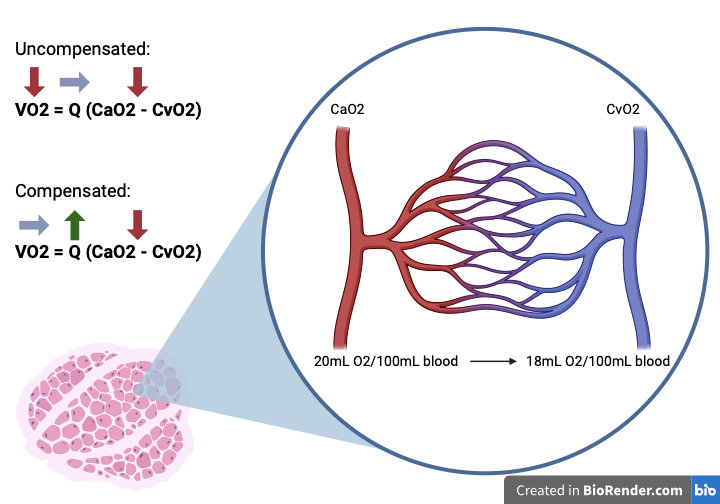
\includegraphics[width=0.5\linewidth]{Sarcopenia.png}
    \caption{Effect of Sarcopenia on avO2 Difference }
    \label{fig:enter-label}
\end{figure}

\textbf{Integrative Exercise: Adaptive Changes in Patients with Anemia }
Use Fick’s Equation to explain the adaptive changes seen in anemic patients.

Anemia is described as a decrease in red blood cell parameters (e.g. RBC count, hemoglobin, hematocrit). Arising from two primary mechanisms: (1) decreased red blood cell production or (2) increased red blood cell loss, anemia can result in cell hypoxia and if severe, tissue anoxia with subsequent cell death. Clinically, patient's with anemia may present with increased baseline levels of fatigue, weakness, tachycardia, and dyspnea.

As previously stated in the text, hemoglobin is a protein present in the RBC’s, which enables the binding and transportation of oxygen to relevant areas of need (both peripheral and visceral tissue). As anemia progresses there is a gradual decline in the blood’s ability to meet the oxygen demands of the tissue. To meet the oxygen demands of the tissue, multi-system compensations are seen. Short term compensations may arise in the form of tachycardia, which would pump more blood (mL) per unit of time in an attempt to adjust for the decrease in oxygenated blood. This increase in heart rate would contribute to an increase in stroke volume and thus, cardiac output. Although this compensatory mechanism may assist in managing local ischemia in the short term, the long term consequences of a chronic increase in cardiac output has significant implications. 



Anemia, which results in low RBC

May clinically present with pallor, increased baseline levels of fatigue, and dyspnea. 

Increased physical activity increases the demand for oxygen. 

Chronic anemia, greater need for oxygen systemically may result in cardiac output increases, but an inverse relationship with exercise tolerance. 

\begin{itemize}
    \item Low CO: hypovolemia, hypoperfusion, shock, arrhythmia, severe metabolic acidosis 
    \item High CO: hypoxia, use of positive inotropy, anemia 
    \item Low SV: High SV: bradycardia, the use of positive inotropes, decreases in afterload 
\end{itemize}


An example provided earlier in the chapter outlined the normal physiologic response to a supine to sit transfer. 

Summary: 




\section{Attain-Sustain Spectrum}

The attain-sustain spectrum in the context of Fick's equation can be described as the relationship between oxygen delivery and oxygen consumption in which the metabolic demands of the tissues are initially met, and then subsequently continued at levels physiologically safe. 

attain - achieving of threshold
sustain 

The body's ultimate goal is preservation of this balance between oxygen delivery and oxygen consumption. 

Fick's equation gives the physical therapist improved insight as it relates to overall understanding of cardiac function, principally, oxygen consumption, flow rate, and arterovenous difference. 

\printbibliography[heading=subbibintoc]